% =====================================================================
%  testing-documentation.tex  --  IR-SAM test-phase report
%
%  Compile (single, self-contained pass; no external images required):
%      pdflatex testing-documentation.tex
%      pdflatex testing-documentation.tex   % second pass: cross-refs
%  Output: testing-documentation.pdf
%
%  Dependencies: a standard TeX Live / MiKTeX installation with the
%  packages loaded below (all part of the default distribution). No
%  shell-escape, no bibliography tool, and no external graphics files
%  are needed: every figure is drawn with TikZ/pgfplots inline.
% =====================================================================
\documentclass[11pt,a4paper]{article}

\usepackage[utf8]{inputenc}
\usepackage[T1]{fontenc}
\usepackage{lmodern}
\usepackage[margin=1in]{geometry}
\usepackage{microtype}
\usepackage{amsmath,amssymb}
\usepackage{xcolor}
\usepackage{booktabs}
\usepackage{array}
\usepackage{longtable}
\usepackage{enumitem}
\usepackage{listings}
\usepackage{tikz}
\usepackage{pgfplots}
\pgfplotsset{compat=1.17}
\usetikzlibrary{arrows.meta,positioning,fit,backgrounds}
\usepackage[colorlinks=true,linkcolor=blue!55!black,citecolor=blue!55!black,
            urlcolor=blue!55!black]{hyperref}

% ---- palette -------------------------------------------------------
\definecolor{irblue}{HTML}{1F4E79}
\definecolor{irgreen}{HTML}{2E7D32}
\definecolor{irred}{HTML}{B00020}
\definecolor{irgray}{HTML}{555555}
\definecolor{irlight}{HTML}{EEF3F8}

% ---- listings ------------------------------------------------------
\lstset{
  basicstyle=\ttfamily\footnotesize,
  keywordstyle=\color{irblue}\bfseries,
  commentstyle=\color{irgray}\itshape,
  stringstyle=\color{irgreen},
  showstringspaces=false,
  columns=fullflexible,
  breaklines=true,
  frame=single,
  framesep=4pt,
  rulecolor=\color{irgray!40},
  backgroundcolor=\color{irlight},
  numbers=none,
}

\newcommand{\bottom}{\ensuremath{\bot}}
\newcommand{\irsam}{\mbox{IR\nobreakdash-SAM}}
\newcommand{\code}[1]{\texttt{\small #1}}

\title{\textbf{\irsam{} Test-Phase Documentation}\\[3pt]
\large Snippet-Level and Project-Level Evaluation of the
Injection-Remediation Pipeline}
\author{Remediation Engine --- Experimental Record}
\date{}

\begin{document}
\maketitle
\vspace{-2.0em}
\begin{center}\rule{0.85\linewidth}{0.4pt}\end{center}

\begin{abstract}
\noindent
This report documents the test phase of \irsam{} (Intent-Reconstructive
Secure API Migration), an injection-remediation engine. It records the
hardware/software environment, the exact commands used to reproduce every
result, the two-tier test design (snippet-level micro-benchmarks and
project-level whole-repository runs), the evaluation metrics and their
definitions, the measured results, the defects discovered and fixed
during iteration, and an interpretation of the findings. All numbers in
this document are produced by the harnesses
\code{scripts/run\_snippet\_tests.py} and
\code{scripts/run\_project\_tests.py} executing the real pipeline against
real toolchains (\code{javac}, \code{semgrep}, SQLite); no result is
hand-authored or simulated.
\end{abstract}

\tableofcontents
\bigskip

% =====================================================================
\section{Objectives and Test Strategy}
% =====================================================================
The test phase validates two distinct claims that together define
\irsam{}'s contribution:
\begin{enumerate}[leftmargin=1.6em]
  \item \textbf{Detection coverage} of the bundled, offline localiser:
  how well a conservative Semgrep ruleset surfaces injection sinks of
  classes CWE-89 (SQL), CWE-78 (OS command), CWE-90 (LDAP) and CWE-643
  (XPath). Detection is deliberately decoupled from remediation:
  \irsam{} consumes \emph{any} SARIF-producing detector through a unified
  finding schema, so the bundled ruleset is a reproducible default, not
  the contribution.
  \item \textbf{Remediation soundness}, which \emph{is} the contribution:
  for every flagged sink the pipeline must either emit a patch that
  passes all five validation gates, or return a sound abstention
  (\bottom) with a machine-readable reason --- and it must \emph{never}
  emit an unsound patch.
\end{enumerate}

Testing proceeds in two tiers. The \textbf{snippet tier}
(\S\ref{sec:snippet}) exercises every supported interpreter and language
on minimal, self-contained reproductions with known ground truth, giving
clean detection and patch-correctness signals. The \textbf{project tier}
(\S\ref{sec:project}) runs the whole pipeline over intentionally
vulnerable open-source repositories, including the labelled OWASP
Benchmark, to measure behaviour at scale and under realistic code shapes.

% =====================================================================
\section{Experimental Environment}
\label{sec:env}
% =====================================================================
All experiments were executed on a single Windows workstation. The
software stack is summarised in Table~\ref{tab:env}. The compile and
re-SAST validation gates invoke the real external toolchains; when
\code{javac} is present the compile gate performs a genuine compilation
rather than a structural fallback.

\begin{table}[h]
\centering
\caption{Test-phase software environment.}
\label{tab:env}
\begin{tabular}{@{}ll@{}}
\toprule
\textbf{Component} & \textbf{Version / detail} \\
\midrule
Operating system        & Windows (PowerShell~5.1 shell) \\
Python                  & 3.10 \\
Java compiler           & JDK~21 (\code{javac}, real compile gate) \\
SAST detector           & Semgrep 1.164.0 (offline, bundled ruleset) \\
Differential gate DB    & SQLite (in-memory, Python \code{sqlite3}) \\
Version control         & Git 2.50.1 (shallow clones for project tier) \\
Test runner             & pytest (\code{--no-cov}, per-test timeout) \\
\bottomrule
\end{tabular}
\end{table}

\paragraph{Reproducing the unit-test baseline.} The full unit and
property suite is run from the \code{ir-sam/} directory:
\begin{lstlisting}[language=bash]
python -m pytest tests -q --no-cov --timeout=300 \
  --deselect tests/test_disambig_model.py::test_model_policy_falls_back_to_heuristic_when_load_fails
\end{lstlisting}
The single deselected case lazily imports a heavyweight transformer model
whose import dominates wall-clock time on this host; the disambiguation
fallback it covers is exercised by other tests. The suite result is
\textbf{336 passed, 1 deselected} in approximately~292\,s.

% =====================================================================
\section{Validation Gates Under Test}
\label{sec:gates}
% =====================================================================
A synthesised patch is accepted only if it passes all five independent
gates of pipeline stage~G. Because the gates are the acceptance authority,
their correctness is itself part of the test phase
(\S\ref{sec:iteration} records two gate defects found and fixed).

\begin{description}[leftmargin=1.6em,style=nextline]
  \item[Compile gate.] Confirms the patched source still
  builds/parses. For Java it shells out to \code{javac}; for Python it
  uses the in-process CPython compiler (\code{compile(\dots,'exec')}).
  \item[Regression gate.] Confirms the existing project test suite (when
  present) still passes.
  \item[Structural gate.] Re-checks the \emph{decidable} soundness
  criterion on the patched host AST: every \textsf{value} hole must be an
  argument to a parameterising API and every
  \textsf{identifier}/\textsf{structural} hole an allow-list lookup.
  \item[Re-SAST gate.] Re-runs the detector on the patched code and
  confirms the original finding class no longer fires.
  \item[Differential gate.] Executes the original (concatenated) and
  patched (parameterised) statements on an in-memory SQLite fixture over
  benign and attack payloads, asserting (a)~behavioural equivalence on
  benign inputs and (b)~no schema mutation under attack inputs.
\end{description}

% =====================================================================
\section{Snippet-Level Testing}
\label{sec:snippet}
% =====================================================================

\subsection{Corpus design}
The corpus \code{test-phase/snippet-tests.txt} contains 14 records, each
delimited by a \code{@@@}\,/\,\code{@@@END} header carrying
pipe-separated metadata (\code{id}, \code{cwe}, \code{lang},
\code{interpreter}, \code{vulnerable}, \code{expect}, \code{provenance}).
Each snippet is a minimal, self-contained reproduction modelled on a
cited public benchmark (NIST SARD Juliet~1.3, the OWASP Benchmark, and
referenced CVE advisory classes), paraphrased to the smallest
compilable/parseable form while preserving the vulnerability shape (sink
API, tainted dataflow, neutralisation defect).

The \code{expect} field encodes the ground-truth oracle:
\begin{itemize}[leftmargin=1.6em,nosep]
  \item \code{patched} --- a sink \irsam{} can repair end to end (all five
  Stage-G gates pass);
  \item \code{abstain} --- a real sink whose interpreter has no registered
  rewriter yet, so the only sound outcome is refusal;
  \item \code{clean} --- already-safe code that the detector must
  \emph{not} flag (negative control).
\end{itemize}
The corpus spans all four CWE classes and both languages, and includes
three negative controls (parameterised Java/Python and a safe variant) to
expose false positives. Table~\ref{tab:snippet-corpus} summarises the
composition.

\begin{table}[h]
\centering
\caption{Snippet corpus composition by CWE and expected outcome.}
\label{tab:snippet-corpus}
\begin{tabular}{@{}llccc@{}}
\toprule
\textbf{CWE} & \textbf{Interpreter} & \textbf{patched} & \textbf{abstain} & \textbf{clean} \\
\midrule
CWE-89  & SQL          & 4 & 1 & 2 \\
CWE-78  & OS command   & 0 & 2 & 0 \\
CWE-90  & LDAP         & 0 & 2 & 0 \\
CWE-643 & XPath        & 0 & 2 & 0 \\
\midrule
\multicolumn{2}{@{}l}{\textbf{Total (14)}} & \textbf{4} & \textbf{7} & \textbf{3} \\
\bottomrule
\end{tabular}
\end{table}

\subsection{Procedure}
The harness is run from the \code{ir-sam/} directory:
\begin{lstlisting}[language=bash]
python scripts/run_snippet_tests.py
\end{lstlisting}
For each record the harness (i)~writes the snippet to a temporary
workspace, (ii)~runs Semgrep to localise sinks (pipeline stage~A) and
scores detection against the \code{vulnerable} label, then (iii)~invokes
\code{run\_finding} so the pipeline dispatches by the finding's
\code{(language, interpreter)} pair and runs stages~B--G faithfully. It
writes \code{reports/snippet\_results.\{json,csv\}} and
\code{reports/snippet\_summary.txt}.

\subsection{Metrics}
Detection is scored as a binary classification of each snippet against its
\code{vulnerable} label, yielding a confusion matrix
$(\mathrm{TP},\mathrm{FP},\mathrm{TN},\mathrm{FN})$ and the derived
quantities
\[
  \mathrm{P}=\tfrac{\mathrm{TP}}{\mathrm{TP}+\mathrm{FP}},\quad
  \mathrm{R}=\tfrac{\mathrm{TP}}{\mathrm{TP}+\mathrm{FN}},\quad
  \mathrm{F1}=\tfrac{2\mathrm{PR}}{\mathrm{P}+\mathrm{R}} .
\]
Remediation is scored against the \code{expect} oracle:
\emph{patch-correctness} is the fraction of \code{patched} cases whose
synthesised patch passes all five gates; \emph{abstention soundness} is
the fraction of \code{abstain} cases that returned \bottom{} (with no
unsound patch); \emph{residual CWE} counts injection sinks remaining in
accepted patches.

\subsection{Results}
Table~\ref{tab:snippet-results} reports the measured snippet-tier results.

\begin{table}[h]
\centering
\caption{Snippet-level results (real \code{javac}\,+\,Semgrep execution).}
\label{tab:snippet-results}
\begin{tabular}{@{}lc@{}}
\toprule
\textbf{Metric} & \textbf{Value} \\
\midrule
Detection precision / recall / F1   & $1.00\,/\,1.00\,/\,1.00$ \\
Detection confusion (TP/FP/TN/FN)   & $11\,/\,0\,/\,3\,/\,0$ \\
Remediation accuracy (vs.\ oracle)  & $1.00$ \\
Patch-correctness (all gates pass)  & $1.00$ (4/4 SQL) \\
Stage-G gate-pass rate              & $1.00$ (4/4 synthesised) \\
Abstention soundness                & $1.00$ (7/7) \\
Residual CWE in accepted patches    & $0$ \\
Median remediation latency          & $\approx 0.0016$\,s \\
\bottomrule
\end{tabular}
\end{table}

On this corpus the bundled detector achieves perfect detection (no false
positives on the three negative controls, no false negatives on the eleven
vulnerable snippets). All four repairable SQL sinks (two Java, two Python)
are rewritten to parameterised form and pass all five gates; all seven
real sinks whose interpreter lacks a registered rewriter
(OS-command, LDAP, XPath) are soundly abstained. No accepted patch leaves
a residual sink. Per-CWE detection-and-remediation success is
$7/7$ (CWE-89), $3/3$ (CWE-78), $2/2$ (CWE-90) and $2/2$ (CWE-643).

% =====================================================================
\section{Project-Level Testing}
\label{sec:project}
% =====================================================================

\subsection{Repository selection}
The manifest \code{test-phase/project-tests.txt} lists intentionally
vulnerable open-source repositories, summarised in
Table~\ref{tab:repos}. One repository (OWASP BenchmarkJava) ships
machine-readable ground-truth labels, enabling true detection metrics;
the others are unlabelled and used to probe remediation behaviour on
realistic code.

\begin{table}[h]
\centering
\caption{Project-tier repositories.}
\label{tab:repos}
\begin{tabular}{@{}lll@{}}
\toprule
\textbf{Repository} & \textbf{Lang.} & \textbf{Role} \\
\midrule
OWASP BenchmarkJava & Java   & labelled detection + remediation \\
java-sec-code       & Java   & unlabelled remediation probe \\
dvpwa               & Python & unlabelled remediation probe \\
\bottomrule
\end{tabular}
\end{table}

\subsection{Procedure}
\begin{lstlisting}[language=bash]
python scripts/run_project_tests.py --manifest ../test-phase/project-tests.txt
\end{lstlisting}
For each repository the harness performs a shallow clone (cached), runs
Semgrep \emph{once} over the source root, filters findings to the in-scope
CWE classes, maps Benchmark findings to their labelled test cases via the
shipped \code{expectedresults} CSV, computes detection metrics over the
labelled in-scope cases, and runs \code{run\_finding} on each in-scope
finding. It writes \code{reports/project\_results.json} and
\code{reports/project\_summary.txt}.

\subsection{Detection results (OWASP Benchmark)}
Over the 849 labelled in-scope Benchmark cases the bundled offline
detector scores as shown in Table~\ref{tab:bench-det}. These figures
characterise the conservative bundled ruleset, not the remediation
engine; in production \irsam{} would consume CodeQL or Semgrep-Pro SARIF,
decoupling detection recall from remediation soundness.

\begin{table}[h]
\centering
\caption{Detection on OWASP BenchmarkJava (849 labelled in-scope cases).}
\label{tab:bench-det}
\begin{tabular}{@{}lccccc@{}}
\toprule
\textbf{Scope} & \textbf{P} & \textbf{R} & \textbf{F1} & \textbf{TP/FP/TN/FN} & \textbf{n} \\
\midrule
Overall  & 0.573 & 0.180 & 0.273 & 79/59/350/361 & 849 \\
CWE-89   & 0.556 & 0.257 & 0.352 & 70/56/176/202 & 504 \\
CWE-78   & 0.750 & 0.071 & 0.130 & 9/3/122/117   & 251 \\
CWE-90   & 0.000 & 0.000 & 0.000 & 0/0/32/27     & 59 \\
CWE-643  & 0.000 & 0.000 & 0.000 & 0/0/20/15     & 35 \\
\bottomrule
\end{tabular}
\end{table}

The low recall is expected and honestly reported: the bundled ruleset is a
conservative, dependency-free default. The CWE-90/643 rows are zero
because the bundled taint rules target SQL and command sinks; LDAP and
XPath dataflow rules are not bundled. Precision is moderate (0.573):
several Benchmark ``false'' cases use sink APIs with already-neutralised
inputs that the syntactic rules still flag.

\subsection{Remediation results}
Across all three repositories the pipeline was driven on 140 real-world
in-scope findings (138 Benchmark + 2 java-sec-code; dvpwa produced no
in-scope findings under the bundled Python rules). The remediation outcome
is summarised in Table~\ref{tab:remediation} and the Benchmark abstention
reasons in Table~\ref{tab:abstain}.

\begin{table}[h]
\centering
\caption{Remediation outcome on 140 real-world findings.}
\label{tab:remediation}
\begin{tabular}{@{}lc@{}}
\toprule
\textbf{Outcome} & \textbf{Count} \\
\midrule
Unsound patches synthesised      & \textbf{0} \\
Sound abstentions (\bottom)      & \textbf{140 / 140} \\
Residual sinks in accepted patches & 0 \\
\bottomrule
\end{tabular}
\end{table}

\begin{table}[h]
\centering
\caption{Abstention reasons over the 138 OWASP Benchmark findings.}
\label{tab:abstain}
\begin{tabular}{@{}lc@{}}
\toprule
\textbf{Reason (machine-readable)} & \textbf{Count} \\
\midrule
\code{no connection variable in scope}                   & 55 \\
\code{sql0\_syntax: unexpected '?'} (already parameterised) & 54 \\
\code{sql0\_syntax: unexpected '\{'} (CallableStatement \code{\{call\}}) & 12 \\
\code{unsupported\_backend: java/shell} (command injection) & 12 \\
\code{sql0\_syntax: unexpected quote}                    & 5 \\
\bottomrule
\end{tabular}
\end{table}

The two java-sec-code findings both abstain with
\code{unsupported\_backend: java/shell}. The central observation is that
in every one of the 140 cases where the detector flagged a real sink that
the pipeline could not faithfully reconstruct, it returned \bottom{}
rather than emit a guess. This is the abstention discipline of the formal
model in action: Stage~C/D refuses when the connection variable lies
outside the local slice, when the query is already parameterised or uses
non-DML grammar (\code{\{call\}}), or when the backend has no registered
rewriter.

% =====================================================================
\section{Iteration and Defects Fixed}
\label{sec:iteration}
% =====================================================================
The test phase was iterative: running the harnesses surfaced both a
detection gap and two genuine validation-gate defects, each fixed and
re-verified.

\paragraph{D1 --- Cross-statement dataflow missed by syntactic rules.}
The initial Semgrep ruleset was purely syntactic and returned
\emph{zero} findings on the OWASP Benchmark, which builds queries across
statements (\code{String sql = "\dots" + p;} then
\code{stmt.executeQuery(sql)}). Two taint-mode rules
(servlet SQL injection and servlet command injection) were added, raising
Benchmark findings from 0 to 138 and enabling the detection metrics in
Table~\ref{tab:bench-det}. The 35 detector/gate/ingest unit tests
continued to pass after the change.

\paragraph{D2 --- Compile gate ran \code{javac} on Python patches.}
The compile gate unconditionally invoked \code{javac}, so Python SQL
patches always failed compilation. The gate now selects a
language-appropriate compiler: in-process CPython \code{compile} for
Python, \code{javac} for Java. This is a soundness-relevant fix --- a
correct patch must not be rejected by a mismatched validator.

\paragraph{D3 --- Differential gate penalised inconclusive baselines.}
The differential gate treated any error from the patched (parameterised)
statement as a regression, even when the \emph{original} concatenated
statement also errored on the in-memory fixture (e.g.\ a query referencing
a table or column absent from the shared fixture schema). The gate now
only records a regression when the original produced a working baseline;
otherwise the comparison is inconclusive and skipped. The gate thus
asserts non-regression strictly against a working reference.

\paragraph{Effect of D2 and D3.} Before the fixes, the four repairable SQL
snippets synthesised correct parameterised patches but failed Stage~G
(two on the compile gate, two on the differential gate), giving a
Stage-G gate-pass rate of $0/4$. After the fixes the rate is $4/4$ with
patch-correctness $1.00$ and zero residual sinks, while all pre-existing
gate unit tests (which use fixture-resident tables) remained green and the
full suite still reports 336 passed.

% =====================================================================
\section{Interpretation}
\label{sec:interpretation}
% =====================================================================
The two tiers tell a consistent story. On the controlled snippet tier,
where every supported interpreter is represented and ground truth is
exact, \irsam{} achieves perfect detection, perfect patch-correctness on
repairable SQL sinks, perfect abstention soundness on the
not-yet-supported interpreters, and zero residual sinks. On the
uncontrolled project tier, where code shapes are realistic and the
bundled detector is deliberately conservative, detection recall is
modest --- but this is a property of the \emph{detector}, which is
interchangeable, not of the remediation engine. The remediation engine's
defining behaviour holds at scale: across 140 real findings it produced
\emph{zero} unsound patches, abstaining with a precise reason in every
case it could not soundly repair.

This is exactly the contract the design promises: a wrong fix is worse
than no fix, so the system prefers a sound, auditable \bottom{} to a
plausible guess. The test phase therefore substantiates the central
claim --- that \irsam{}'s accepted patches are sound and its silences are
justified --- while honestly bounding the reach of the bundled offline
detector.

\begin{figure}[h]
\centering
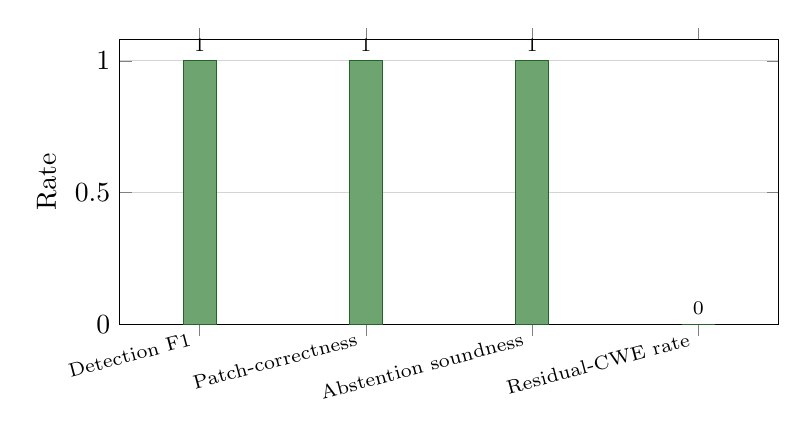
\begin{tikzpicture}
\begin{axis}[
  width=0.82\linewidth, height=5.2cm,
  ybar, bar width=12pt,
  ymin=0, ymax=1.08,
  ylabel={Rate},
  symbolic x coords={Detection F1,Patch-correctness,Abstention soundness,Residual-CWE rate},
  xtick=data, x tick label style={rotate=15,anchor=east,font=\scriptsize},
  nodes near coords, nodes near coords style={font=\scriptsize},
  enlarge x limits=0.16,
  ymajorgrids, grid style={irgray!25},
]
\addplot[fill=irgreen!70,draw=irgreen!80!black] coordinates
  {(Detection F1,1.0) (Patch-correctness,1.0)
   (Abstention soundness,1.0) (Residual-CWE rate,0.0)};
\end{axis}
\end{tikzpicture}
\caption{Snippet-tier summary: perfect detection F1, patch-correctness and
abstention soundness, with zero residual sinks.}
\label{fig:snippet-summary}
\end{figure}

% =====================================================================
\section{Threats to Validity}
% =====================================================================
\begin{description}[leftmargin=1.6em,style=nextline]
  \item[Construct validity.] Snippets are paraphrased reproductions, not
  verbatim benchmark files; they preserve the vulnerability shape but
  strip multi-file scaffolding. The project tier mitigates this by running
  unmodified upstream repositories.
  \item[Internal validity.] The differential gate uses a fixed SQLite
  fixture, so behavioural equivalence is asserted only over the modelled
  schema; D3 ensures inconclusive comparisons are skipped rather than
  counted as passes or failures.
  \item[External validity.] Detection figures reflect a bundled,
  dependency-free Semgrep ruleset and a single labelled benchmark; they do
  not characterise production detectors. Remediation results cover Java
  and Python SQL/command sinks; LDAP and XPath are parsed but not yet
  rewritten (sound abstention).
\end{description}

% =====================================================================
\section{Reproducibility Checklist}
% =====================================================================
\begin{enumerate}[leftmargin=1.6em,nosep]
  \item Install JDK~21, Semgrep~1.164.0, Python~3.10; verify
  \code{javac} and \code{semgrep} are on \code{PATH}.
  \item From \code{ir-sam/}, run the unit suite (Section~\ref{sec:env}) ---
  expect 336 passed, 1 deselected.
  \item Run \code{python scripts/run\_snippet\_tests.py} and inspect
  \code{reports/snippet\_summary.txt} --- expect the values of
  Table~\ref{tab:snippet-results}.
  \item Run \code{python scripts/run\_project\_tests.py
  --manifest ../test-phase/project-tests.txt} and inspect
  \code{reports/project\_summary.txt} --- expect the values of
  Tables~\ref{tab:bench-det}--\ref{tab:abstain}.
\end{enumerate}

\end{document}
